% !TeX root = ../tesis.tex

\section{Supported Nanoparticles}


\begin{figure}\centering
%\def\svgwidth{\textwidth} \small
%\includeinkscape{2-Results-Figs/redshift/redshift}%
\includegraphics[width = .55\textwidth ]{2-Results-Figs/incidencia-externa/Supported-FEM.pdf}%
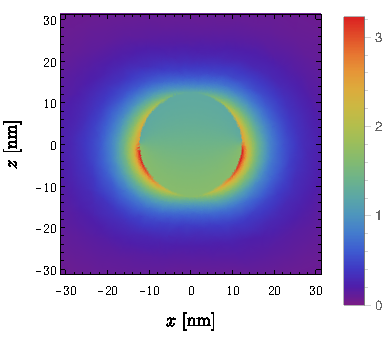
\includegraphics[width = .4\textwidth ]{2-Results-Figs/incidencia-externa/Isolated-COMSOL.pdf}%
\caption[Convergence tests: The Meshing]{Resonance wavlength ($\lambda_\text{res}$) of the scattering (orange) and extinction (black) cross sections as functions of the NPs radii when embedded  \ref{sfig:red:1} into air and \ref{sfig:red:2} into water, and as function of the refractive index of the matrix for NP of radius set to  \ref{sfig:red:3} 12.5 nm and \ref{sfig:red:4} 50 nm.}
\end{figure}




\begin{figure}\centering
%\def\svgwidth{\textwidth} \small
%\includeinkscape{2-Results-Figs/redshift/redshift}%
\includegraphics[width = .9\textwidth ]{2-Results-Figs/incidencia-iterna/normal_internal.png}%
\caption[Convergence tests: The Meshing]{Resonance wavlength ($\lambda_\text{res}$) of the scattering (orange) and extinction (black) cross sections as functions of the NPs radii when embedded  \ref{sfig:red:1} into air and \ref{sfig:red:2} into water, and as function of the refractive index of the matrix for NP of radius set to  \ref{sfig:red:3} 12.5 nm and \ref{sfig:red:4} 50 nm.}
\end{figure}




\begin{figure}\centering
%\def\svgwidth{\textwidth} \small
%\includeinkscape{2-Results-Figs/redshift/redshift}%
\includegraphics[width = .9\textwidth ]{2-Results-Figs/incidencia-iterna/angle_internal_s.png}%
\caption[Convergence tests: The Meshing]{Resonance wavlength ($\lambda_\text{res}$) of the scattering (orange) and extinction (black) cross sections as functions of the NPs radii when embedded  \ref{sfig:red:1} into air and \ref{sfig:red:2} into water, and as function of the refractive index of the matrix for NP of radius set to  \ref{sfig:red:3} 12.5 nm and \ref{sfig:red:4} 50 nm.}
\end{figure}


\section{Incrustaded Nanoparticles}



\begin{figure}\centering
%\def\svgwidth{\textwidth} \small
%\includeinkscape{2-Results-Figs/redshift/redshift}%
\includegraphics[width = .9\textwidth ]{2-Results-Figs/incidencia-iterna/angle_internal_p.png}%
\caption[Convergence tests: The Meshing]{Resonance wavlength ($\lambda_\text{res}$) of the scattering (orange) and extinction (black) cross sections as functions of the NPs radii when embedded  \ref{sfig:red:1} into air and \ref{sfig:red:2} into water, and as function of the refractive index of the matrix for NP of radius set to  \ref{sfig:red:3} 12.5 nm and \ref{sfig:red:4} 50 nm.}
\end{figure}







\begin{figure}\centering
%\def\svgwidth{\textwidth} \small
%\includeinkscape{2-Results-Figs/redshift/redshift}%
\includegraphics[width = .9\textwidth ]{2-Results-Figs/QnormIntExt-inc.png}%
\caption[Convergence tests: The Meshing]{Resonance wavlength ($\lambda_\text{res}$) of the scattering (orange) and extinction (black) cross sections as functions of the NPs radii when embedded  \ref{sfig:red:1} into air and \ref{sfig:red:2} into water, and as function of the refractive index of the matrix for NP of radius set to  \ref{sfig:red:3} 12.5 nm and \ref{sfig:red:4} 50 nm.}
\end{figure}
